% Solution_Template.tex
\documentclass[11pt,a4paper]{article}
\usepackage[utf8]{inputenc}
\usepackage[T1]{fontenc}
\usepackage[ngerman, english]{babel} % remove ngerman if you prefer English only
\usepackage{geometry}
\usepackage{fancyhdr}
\usepackage{hyperref}
\usepackage{tikz}
\usepackage{longtable}
\usepackage{amsmath}
\usepackage{svg}

\geometry{margin=25mm}
\pagestyle{fancy}
\fancyhf{}
\renewcommand{\headrulewidth}{0.4pt}
\lhead{\textbf{Name:} \studentname}
\rhead{\textbf{Matr.-Nr.:} \studentnumber}
\cfoot{\thepage}

% User info - edit these
\newcommand{\studentname}{Matthias Janßen}
\newcommand{\studentnumber}{1871808}
\newcommand{\course}{Übersetzung und Analyse von Programmen}
\newcommand{\institute}{Universität Trier}

\title{\course}
\author{\studentname\\Matrikelnummer: \studentnumber\\\institute}
\date{\today}

\begin{document}

\maketitle

\begin{center}
    \textbf{Abgabe:} Assignment / Sheet \\
    \vspace{4mm}
    \textbf{Betreuer:} Prof. Dr. Stephan Diehl\\Jan Niclas Ruppenthal, M.Sc.
\end{center}

\bigskip

\section*{Aufgaben}
% Start writing your solutions here.

\section{Aufgabe 1}

\begin{figure}[htpb]
    \centering
    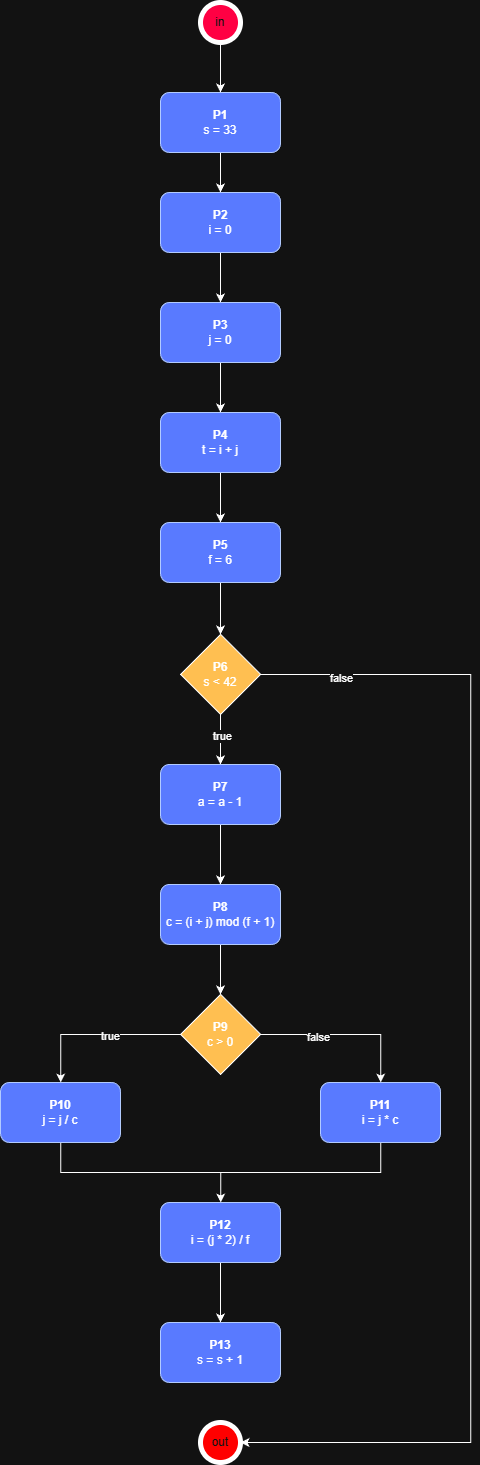
\includegraphics[height=0.8\textheight]{Kontrollflussgraph.png}    
\end{figure}

\newpage
\section{Aufgabe 2}

\subsection*{USE und DEF Mengen}
    \begin{longtable}{| c | c | c |}
    \hline
    v & USE(v) = & DEF(v) = \\
    \hline
    in & $\emptyset$ & $\emptyset$ \\
    \hline
    p1 & $\emptyset$ & \{s\}  \\
    \hline
    p2 & $\emptyset$ & \{i\} \\
    \hline
    p3 & $\emptyset$ & \{j\} \\
    \hline
    p4 & \{i, j\} & \{t\} \\
    \hline
    p5 & $\emptyset$ & \{f\} \\
    \hline
    p6 & \{s\} & $\emptyset$ \\
    \hline
    p7 & \{a\} & \{a\} \\
    \hline
    p8 & \{i, j, f\} & \{c\} \\
    \hline
    p9 & \{c\} & $\emptyset$ \\
    \hline
    p10 & \{j, c\} & \{j\} \\
    \hline
    p11 & \{j, c\} & \{i\} \\
    \hline
    p12 & \{j, f\} & \{i\} \\
    \hline
    p13 & \{s\} & \{s\} \\
    \hline
    out & $\emptyset$ & $\emptyset$ \\
    \hline
\end{longtable}

\subsection*{Live Variable Analyse nach korrekter Formel}

Formel: $\text{OUT}[v] = \bigcup_{(v,s) \in E} \text{IN}[s]$ und $\text{IN}[v] = (\text{OUT}[v] \setminus \text{DEF}[v]) \cup \text{USE}[v]$

\subsubsection*{Initialisierung (Iteration 0)}

    \begin{longtable}{| c | c | c |}
    \hline
    v & IN[v] = USE[v] & OUT[v] \\
    \hline
    in & $\emptyset$ & - \\
    \hline
    p1 & $\emptyset$ & - \\
    \hline
    p2 & $\emptyset$ & - \\
    \hline
    p3 & $\emptyset$ & - \\
    \hline
    p4 & \{i, j\} & - \\
    \hline
    p5 & $\emptyset$ & - \\
    \hline
    p6 & \{s\} & - \\
    \hline
    p7 & \{a\} & - \\
    \hline
    p8 & \{i, j, f\} & - \\
    \hline
    p9 & \{c\} & - \\
    \hline
    p10 & \{j, c\} & - \\
    \hline
    p11 & \{j, c\} & - \\
    \hline
    p12 & \{j, f\} & - \\
    \hline
    p13 & \{s\} & - \\
    \hline
    out & $\emptyset$ & - \\
    \hline
\end{longtable}

\subsubsection*{Iteration 1}

    \begin{longtable}{| c | c | c |}
    \hline
    v & IN[v] & OUT[v] \\
    \hline
    in & $\emptyset$ & $\emptyset$ \\
    \hline
    p1 & $\emptyset$ & $\emptyset$ \\
    \hline
    p2 & $\emptyset$ & $\emptyset$ \\
    \hline
    p3 & \{i\} & \{i, j\} \\
    \hline
    p4 & \{i, j\} & $\emptyset$ \\
    \hline
    p5 & \{s\} & \{s\} \\
    \hline
    p6 & \{s, a\} & \{s, a\} \\
    \hline
    p7 & \{i, j, f, a\} & \{i, j, f\} \\
    \hline
    p8 & \{i, j, f\} & \{c\} \\
    \hline
    p9 & \{j, c\} & \{j, c\} \\
    \hline
    p10 & \{f, j, c\} & \{j, f\} \\
    \hline
    p11 & \{j, f, c\} & \{j, f\} \\
    \hline
    p12 & \{s, j, f\} & \{s\} \\
    \hline
    p13 & \{s\} & \{s\} \\
    \hline
    out & $\emptyset$ & - \\
    \hline
\end{longtable}

\subsubsection*{Iteration 2}

    \begin{longtable}{| c | c | c |}
    \hline
    v & IN[v] & OUT[v] \\
    \hline
    in & $\emptyset$ & $\emptyset$ \\
    \hline
    p1 & $\emptyset$ & $\emptyset$ \\
    \hline
    p2 & $\emptyset$ & \{i\} \\
    \hline
    p3 & \{i\} & \{i, j\} \\
    \hline
    p4 & \{i, j, s, a\} & \{s\} \\
    \hline
    p5 & \{s\} & \{i, j, f, s, a\} \\
    \hline
    p6 & \{i, j, f, s, a\} & \{i, j, f, s, a\} \\
    \hline
    p7 & \{i, j, f, a\} & \{i, j, f\} \\
    \hline
    p8 & \{i, j, f\} & \{f, j, c\} \\
    \hline
    p9 & \{f, j, c\} & \{f, j, c\} \\
    \hline
    p10 & \{s, f, j, c\} & \{s, j, f\} \\
    \hline
    p11 & \{s, j, f, c\} & \{s, j, f\} \\
    \hline
    p12 & \{s, j, f\} & \{i, j, f, s, a\} \\
    \hline
    p13 & \{i, j, f, s, a\} & \{i, j, f, s, a\} \\
    \hline
    out & $\emptyset$ & - \\
    \hline
\end{longtable}

\subsubsection*{Iteration 3}

    \begin{longtable}{| c | c | c |}
    \hline
    v & IN[v] & OUT[v] \\
    \hline
    in & $\emptyset$ & $\emptyset$ \\
    \hline
    p1 & $\emptyset$ & $\emptyset$ \\
    \hline
    p2 & $\emptyset$ & \{i\} \\
    \hline
    p3 & \{i\} & \{i, j\} \\
    \hline
    p4 & \{i, j, s, a\} & \{s\} \\
    \hline
    p5 & \{i, j, s, a\} & \{i, j, f, s, a\} \\
    \hline
    p6 & \{i, j, f, s, a\} & \{i, j, f, s, a\} \\
    \hline
    p7 & \{i, j, f, a\} & \{i, j, f\} \\
    \hline
    p8 & \{i, j, f\} & \{f, j, c\} \\
    \hline
    p9 & \{f, j, c\} & \{f, j, c\} \\
    \hline
    p10 & \{s, f, j, c\} & \{s, j, f\} \\
    \hline
    p11 & \{s, j, f, c\} & \{s, j, f\} \\
    \hline
    p12 & \{i, j, f, s, a\} & \{i, j, f, s, a\} \\
    \hline
    p13 & \{i, j, f, s, a\} & \{i, j, f, s, a\} \\
    \hline
    out & $\emptyset$ & - \\
    \hline
\end{longtable}

\textbf{Ergebnis:} Fixpunkt erreicht in Iteration 3.

\subsection*{Analyse und Algorithmus}

\subsubsection*{Algorithmus nach Vorlesung}

Die Live Variable Analyse folgt der Rückwärts-Analyse:

\begin{enumerate}
    \item \textbf{Initialisierung:} Für alle $v \in V$: $\text{IN}[v] := \text{USE}[v]$, $\text{OUT}[v] := \emptyset$
    \item \textbf{Fixpunkt-Iteration:} Solange sich Werte ändern, für alle $v \in V \setminus \{in\}$:
    \begin{align*}
        \text{OUT}[v] &:= \bigcup_{(v,s) \in E} \text{IN}[s] \\
        \text{IN}[v] &:= (\text{OUT}[v] \setminus \text{DEF}[v]) \cup \text{USE}[v]
    \end{align*}
\end{enumerate}

Die Berechnung terminiert nach endlich vielen Iterationen, da die Mengen nur wachsen können und nach oben beschränkt sind.

\subsubsection*{Interpretazione der Ergebnisse}

Eine Variable $v$ ist an Programmpunkt $p$ \textbf{lebendig} (in $\text{IN}[p]$), wenn:
\begin{itemize}
    \item Sie an $p$ oder einem Nachfolger verwendet wird, ODER
    \item Sie an $p$ definiert wird, aber ihren alten Wert nicht überschreibt (was hier nicht vorkommt)
\end{itemize}

Nach Fixpunkt-Erreichen zeigen die Tabellen folgende lebendigen Variablen:

\begin{itemize}
    \item \textbf{p1-p3:} Initialisierungen, keine lebendig eintretenden Variablen → $\text{IN} = \emptyset$
    \item \textbf{p4:} $t = i + j$: Nur $i, j$ sind lebendig. Variable $t$ ist \textbf{tot}, da nie verwendet.
    \item \textbf{p5:} $f = 6$: Keine eingangsleben Variablen. $f$ wird ausgegeben, aber ist nicht eingangsleben.
    \item \textbf{p6-p13:} Schleifenkörper: Alle Variablen $\{i, j, f, s, a\}$ bleiben lebendig durch Schleifen-Rücksprünge.
\end{itemize}

\subsubsection*{Optimierungsmöglichkeiten}

\textbf{1. Dead Code Elimination:}
\begin{itemize}
    \item Die Zuweisung $t = i + j$ an $p4$ ist \textbf{sicher löschbar}, da $t \notin \text{IN}[p4]$.
    \item Die Variable $t$ wird nach ihrer Definition nie verwendet.
    \item \textbf{Grund:} Keine nachfolgenden Programmpunkte benötigen $t$.
\end{itemize}

\textbf{2. Wirkungslose Zuweisungen im Schleifenkörper:}
\begin{itemize}
    \item Die Zuweisung $a = s - 1$ an $p7$ ist wirkungslos, da $a \notin \text{OUT}[p7]$ (nur $\{i,j,f\}$ werden nach $p7$ benötigt).
    \item Variable $a$ wird in $p7$ definiert, aber nicht in Nachfolgern verwendet.
    \item \textbf{Grund:} $a$ ist an $p7$ \textbf{tot}. Die Zuweisung kann eliminiert werden.
\end{itemize}

\textbf{3. Redundante Berechnung $c = (i+j) \mod (f+1)$:}
\begin{itemize}
    \item Nur die Bedingung $c > 0$ wird genutzt, nicht aber der konkrete Wert von $c$.
    \item Dies ist eine potentielle Optimierungsstelle für spekulativen Code oder Branch-Prediction.
    \item \textbf{Grund:} $c$ ist nach Berechnung lebendig, wird aber primär für Kontrollflussentscheidung genutzt.
\end{itemize}

\subsubsection*{Annotationen des Kontrollflussgraphen}

Der Graph wird mit den Fixpunkt-Werten annotiert:

\begin{center}
\begin{tabular}{|c|c|c|}
\hline
\textbf{Knoten} & \textbf{IN (Eingang)} & \textbf{OUT (Ausgang)} \\
\hline
in & $\emptyset$ & $\emptyset$ \\
\hline
p1-p3 & $\emptyset$ & $\emptyset$ (initiale Zuweisungen) \\
\hline
p4 & $\{i, j, s, a\}$ & $\{s\}$ \\
\hline
p5 & $\{i, j, s, a\}$ & $\{i, j, f, s, a\}$ \\
\hline
p6 (Loop-Test) & $\{i, j, f, s, a\}$ & $\{i, j, f, s, a\}$ \\
\hline
p13 (Loop-Increment) & $\{i, j, f, s, a\}$ & $\{i, j, f, s, a\}$ (Schleife!) \\
\hline
\end{tabular}
\end{center}

Die Schleife p6 → ... → p13 → p6 führt dazu, dass sich lebendige Variablen bis zur Schleife propagieren.

Nach Iteration 3 ändert sich nichts mehr. Jede Variable kennt jetzt alle Variablen, die sie braucht, und die Schleife hat nichts Neues mehr zu bringen. Das heißt: Fixpunkt erreicht.

\end{document}

\end{document}